\documentclass[12pt, titlepage]{article}

\usepackage{graphicx} % Allows for images
\usepackage{wrapfig} % Allows for text wrapping around images
\usepackage{hyperref} % Allows for hyperlinks
\usepackage{siunitx} % Allows for SI units
\usepackage{amsmath} % Allows for math
\usepackage{enumerate} % Allows for custom enumerations
\usepackage{xcolor} % Allows for custom colors
\usepackage{tikz, tcolorbox} % Allows for custom boxes
\usepackage{microtype} % Allows for better text alignment
\usepackage{listings} % Allows for code listings
\usepackage{booktabs} % Allows for better tables
\usepackage{float} % Allows for better figure placement
\usepackage{geometry} % Allows for custom page geometry
\usepackage{fancyhdr} % Allows for custom headers and footers
\usepackage{caption} % Allows for custom captions
\usepackage{array} % Required package for specifying column width and line in the table
\usepackage{changepage} % Required for the adjustwidth environment to temporarily widen margins

\fancypagestyle{myarticlestyle}{
    \fancyhf{} % Clear header and footer
    \fancyhead[L]{\leftmark} % Section name on the left
    \fancyhead[R]{\thepage} % Page number on the right
}
\fancypagestyle{tocstyle}{
    \fancyhf{} % Clear header and footer
    \fancyhead[L]{CONTENTS} % Section name on the left
    \fancyhead[R]{\thepage} % Page number on the right
}

\pagestyle{myarticlestyle}
\setlength{\headheight}{15pt}

\begin{document}
\tableofcontents
\listoffigures
\listoftables
\thispagestyle{tocstyle}
\newpage
\section{Objectives}
The behavior of beams under different loading conditions is a fundamental
aspect of structural engineering. Understanding how beams deflect when
subjected to varying loads is crucial in designing safe and efficient
structures. In this experiment, the focus is on two specific beam
configurations: the cantilever and the simply supported beam. The deflection of
these beams will be investigated both theoretically and experimentally.\\[10pt]
The objectives for this experiment are outlined as follows:
\begin{enumerate}
    \item \textbf{Measurement of Deflection:} Experimentally acquire accurate
      values of deflection for both a cantilever and a simply supported beam
      under varying loads to understand their structural behaviors.
    
    \item \textbf{Comparison of Experimental and Theoretical Results:} Analyze
      and compare the obtained experimental deflection values with the
      theoretically predicted values for both the cantilever and the simply
      supported beam to assess the accuracy and reliability of theoretical
      models in predicting structural deflections.
\end{enumerate}

These objectives aim to provide a comprehensive understanding of how different
types of beam structures behave under applied loads and to evaluate the
alignment between theoretical predictions and actual experimental observations
in real-world scenarios.
\newpage
\section{Procedure}
This experiment consists of two parts: the cantilever beam testing and the
simply supported beam testing.
\subsection{Cantilever Beam Testing}
\begin{enumerate}
    \item \textbf{Step 1:} Check the initial readings of the electrical
      potentiometers to ensure they are zero.
    
    \item \textbf{Step 2:} Apply loads in increments of 2 lb (8.9 N) at the
      mid-span (\(P1\)) up to a total load of 10 lb. Record the vertical
      deflections at both the mid-span (\(P1\)) and at the end of the
      cantilever beam (\(P2\)) for each load.
    
    \item \textbf{Step 3:} Remove the applied load.
    
    \item \textbf{Step 4:} Apply the same set of loads to the end of the beam
      (\(P2\)) and measure the deflections at the mid-span (\(P1\)) and at the
      end of the cantilever beam (\(P2\)).
\end{enumerate}

\subsection{Simply Supported Beam Testing}
\begin{enumerate}
    \item \textbf{Step 1:} Ensure that the initial readings of the electrical
      potentiometers are zero.
    
    \item \textbf{Step 2:} Apply loads in increments of 10 lb (44.482 N) at the
      mid-span of the beam (\(P3\)) up to a total load of 40 lb (177.928 N).
      Record the vertical deflections at both the mid-span (\(P3\)) and at the
      quarter-span of the beam (\(P4\)) for each load.
    
    \item \textbf{Step 3:} Remove the applied load.
    
    \item \textbf{Step 4:} Apply the same set of loads to the quarter-span
      (\(P4\)) and measure the deflections at the mid-span (\(P3\)) and at the
      quarter-span of the beam (\(P4\)).
\end{enumerate}
Throughout the experiment, ensure accurate recording of all measurements,
maintain the safety protocols, and perform the tests as per the specified
loading conditions for each beam configuration.
\newpage
\subsection{Free-Body Diagrams}
This section contains the free-body diagrams for the each beam and each loading
condition.
\subsubsection{Cantilever Beam Load Applied at the Mid-Span}
\begin{figure}[H]
    \centering
    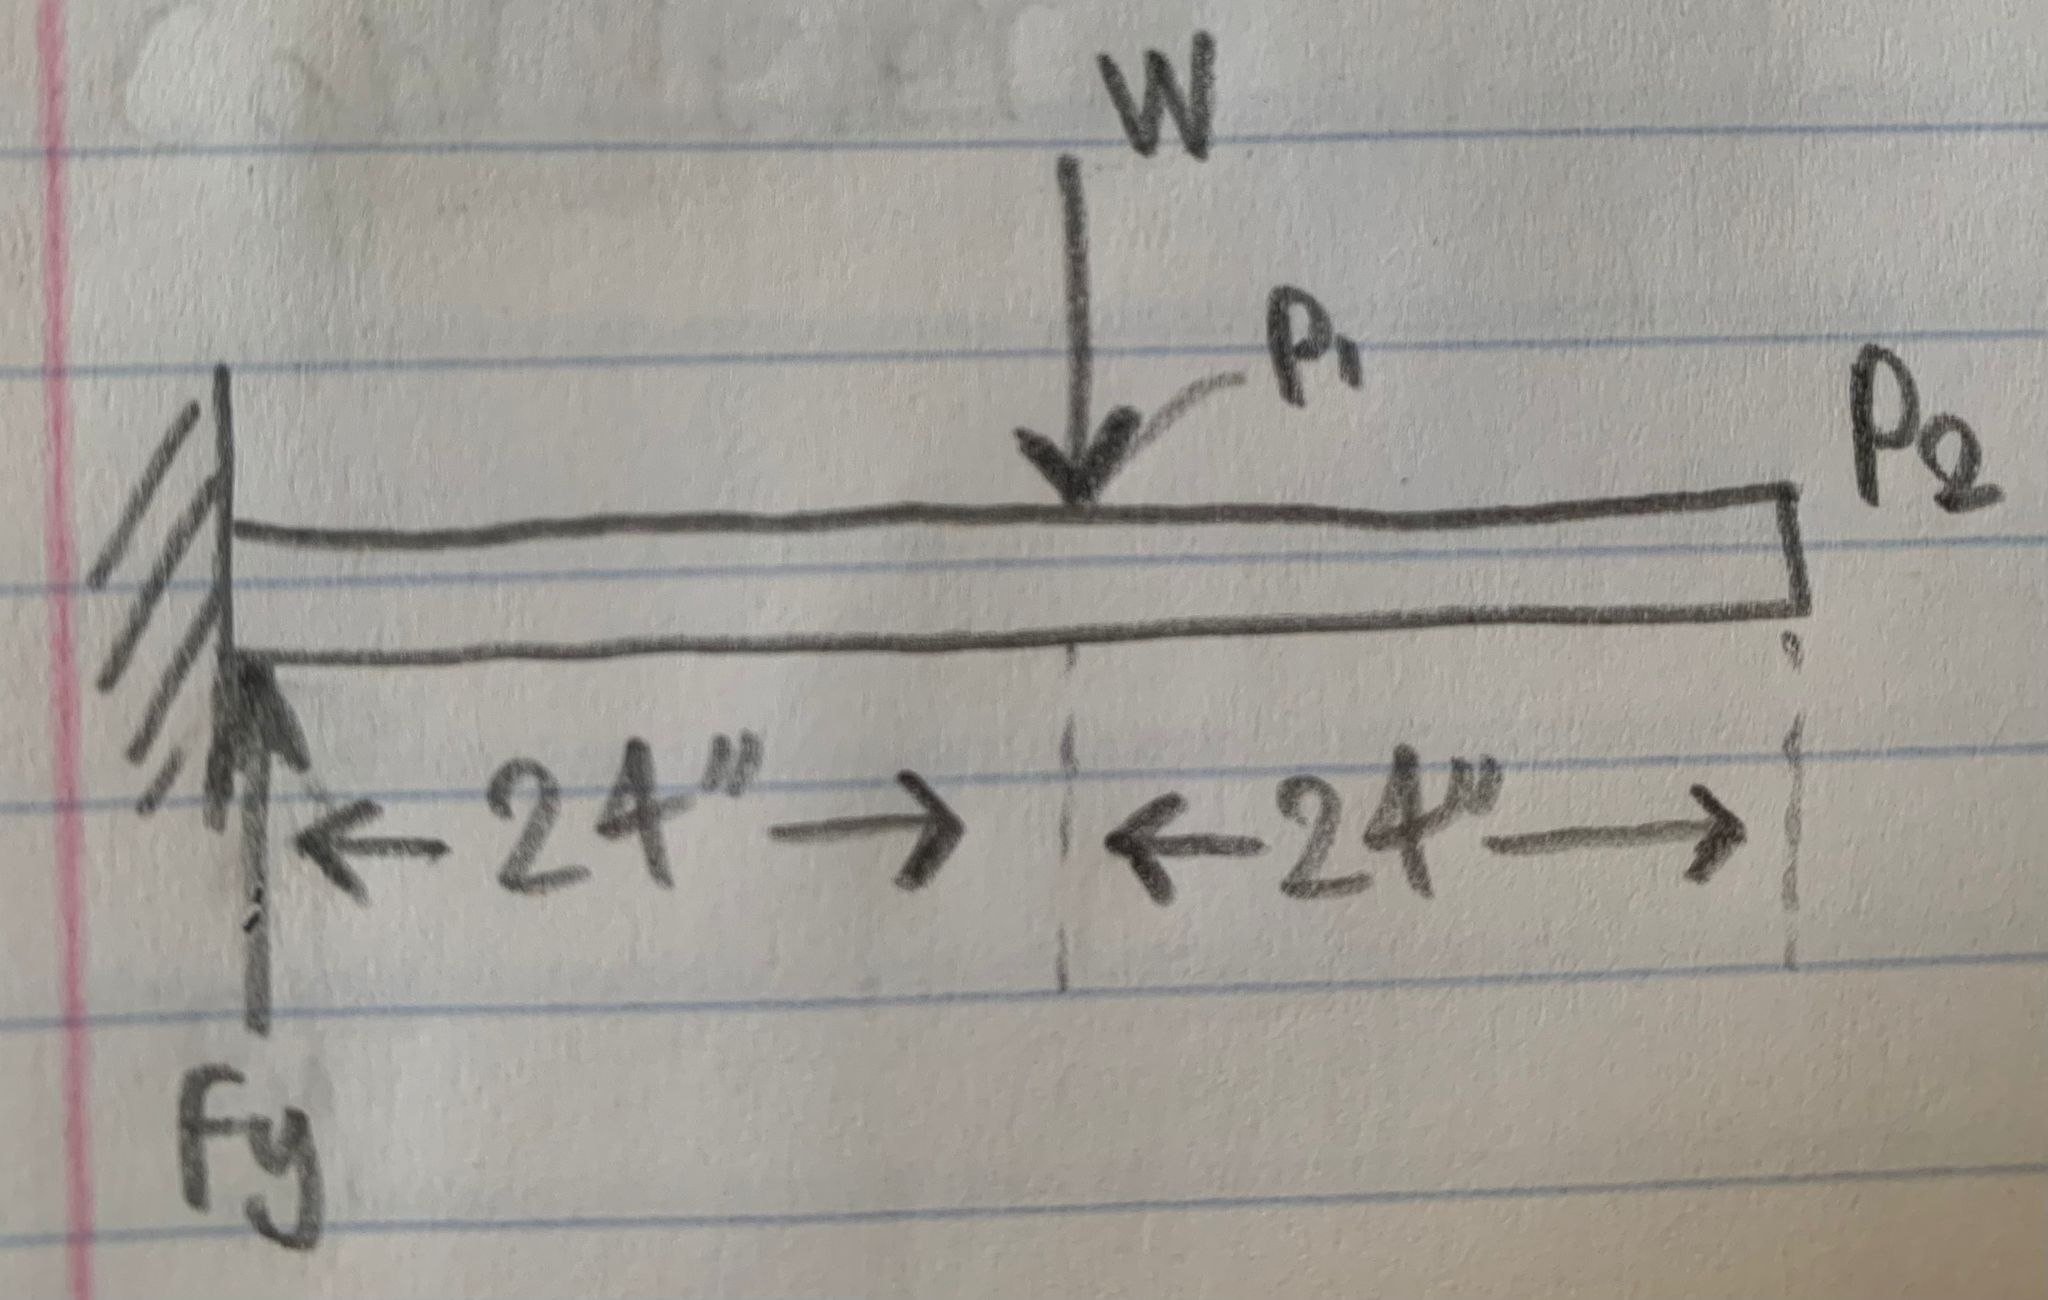
\includegraphics[width=0.6\textwidth]{./Images/C_mid.jpg}
    \caption{Free-body diagram of the cantilever beam with the load applied at
    the mid-span.}
    \label{fig:CantileverBeamMid}
\end{figure}
\subsubsection{Cantilever Beam Load Applied at the End}
\begin{figure}[H]
    \centering
    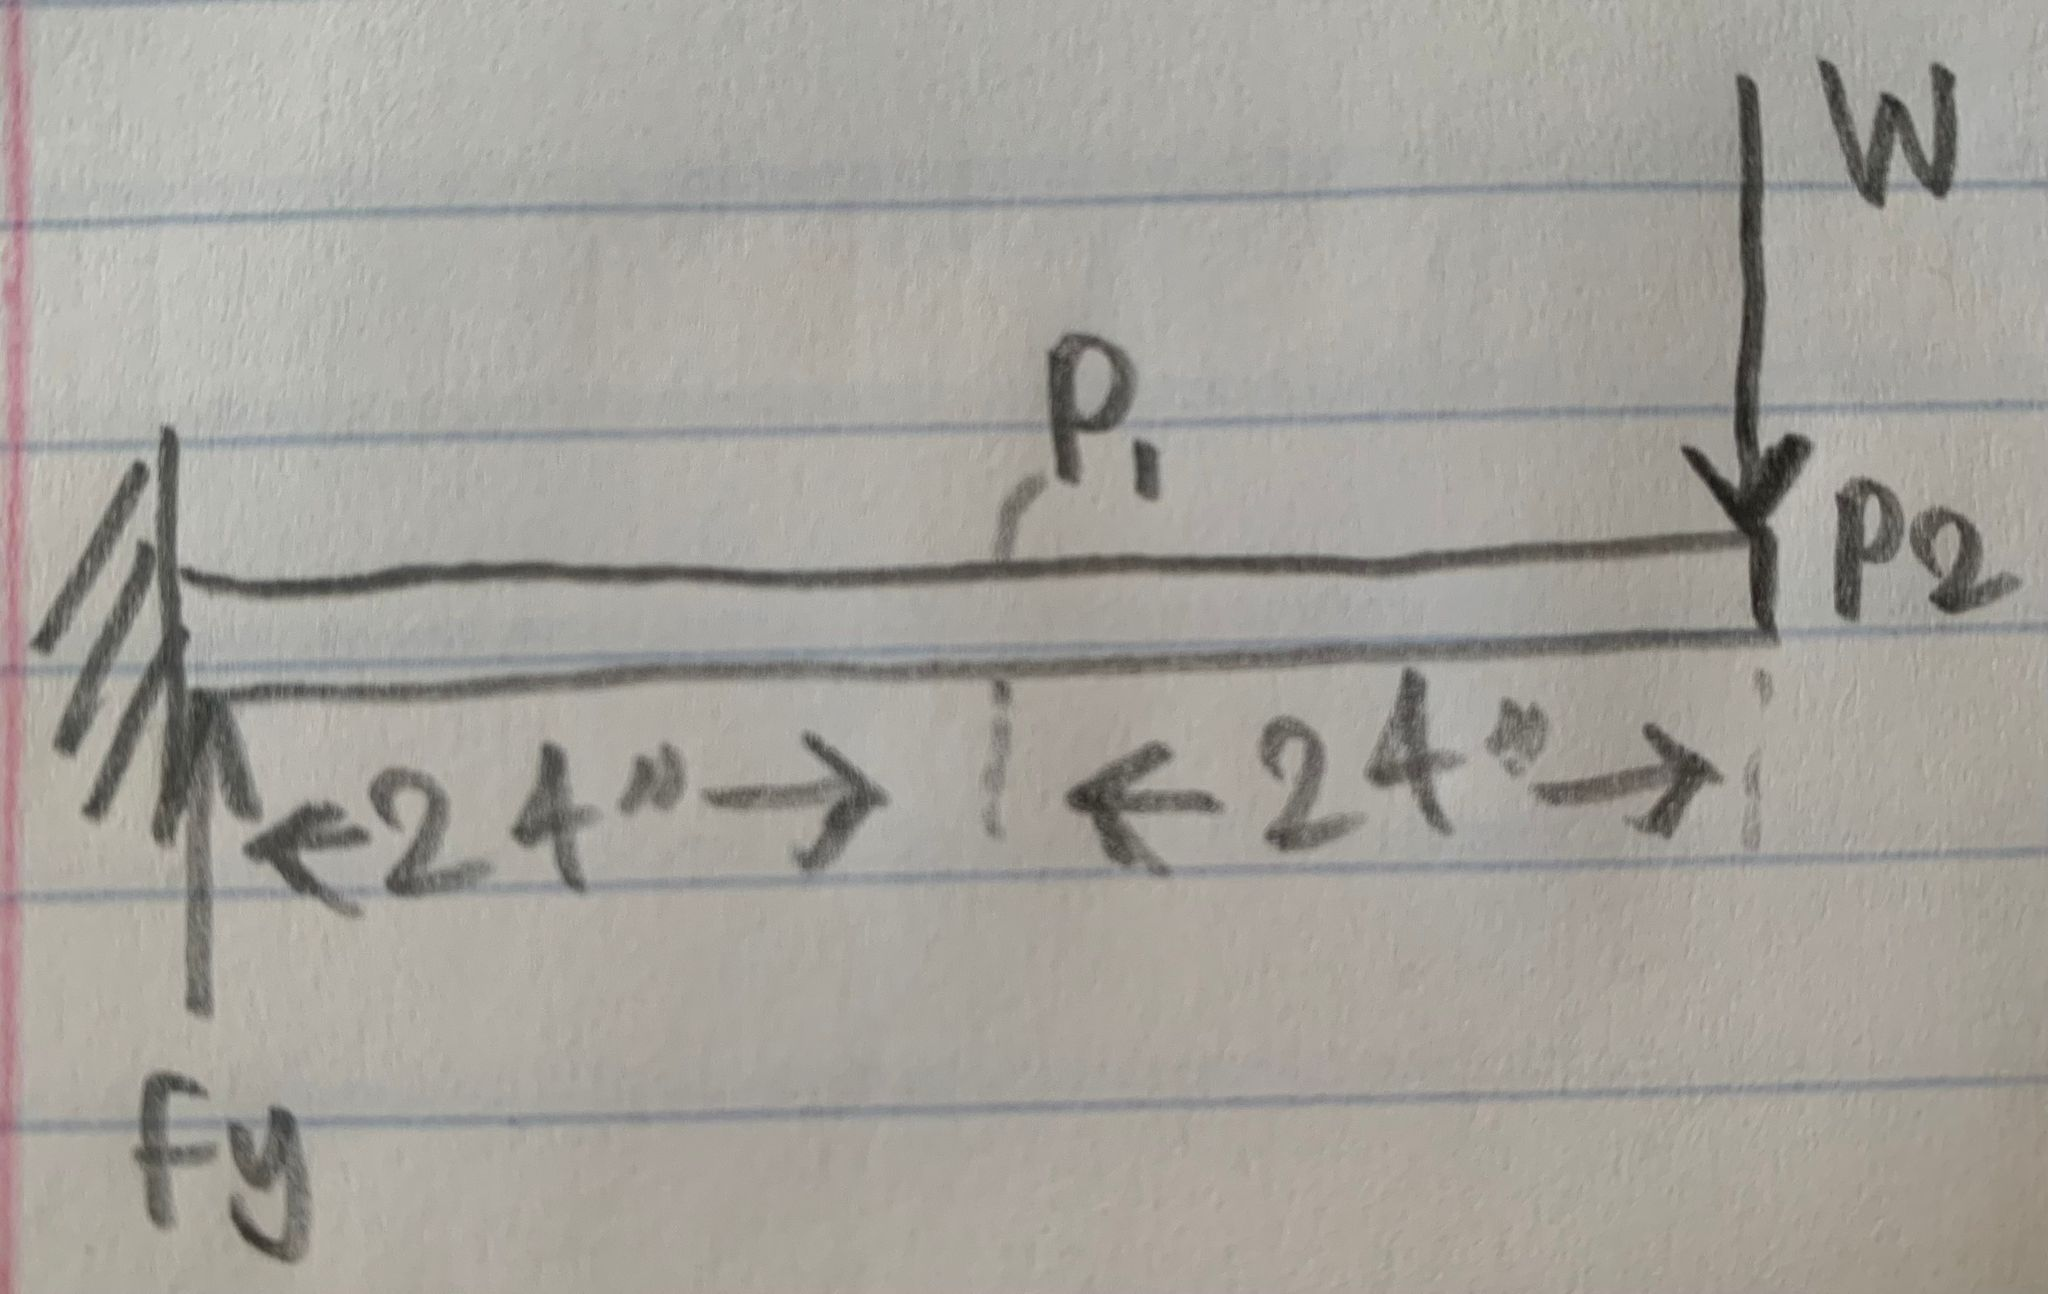
\includegraphics[width=0.6\textwidth]{./Images/C_end.jpg}
    \caption{Free-body diagram of the cantilever beam with the load applied at
    the end.}
    \label{fig:CantileverBeamEnd}
\end{figure}
\subsubsection{Simply Supported Beam Load Applied at the Mid-Span}
\begin{figure}[H]
    \centering
    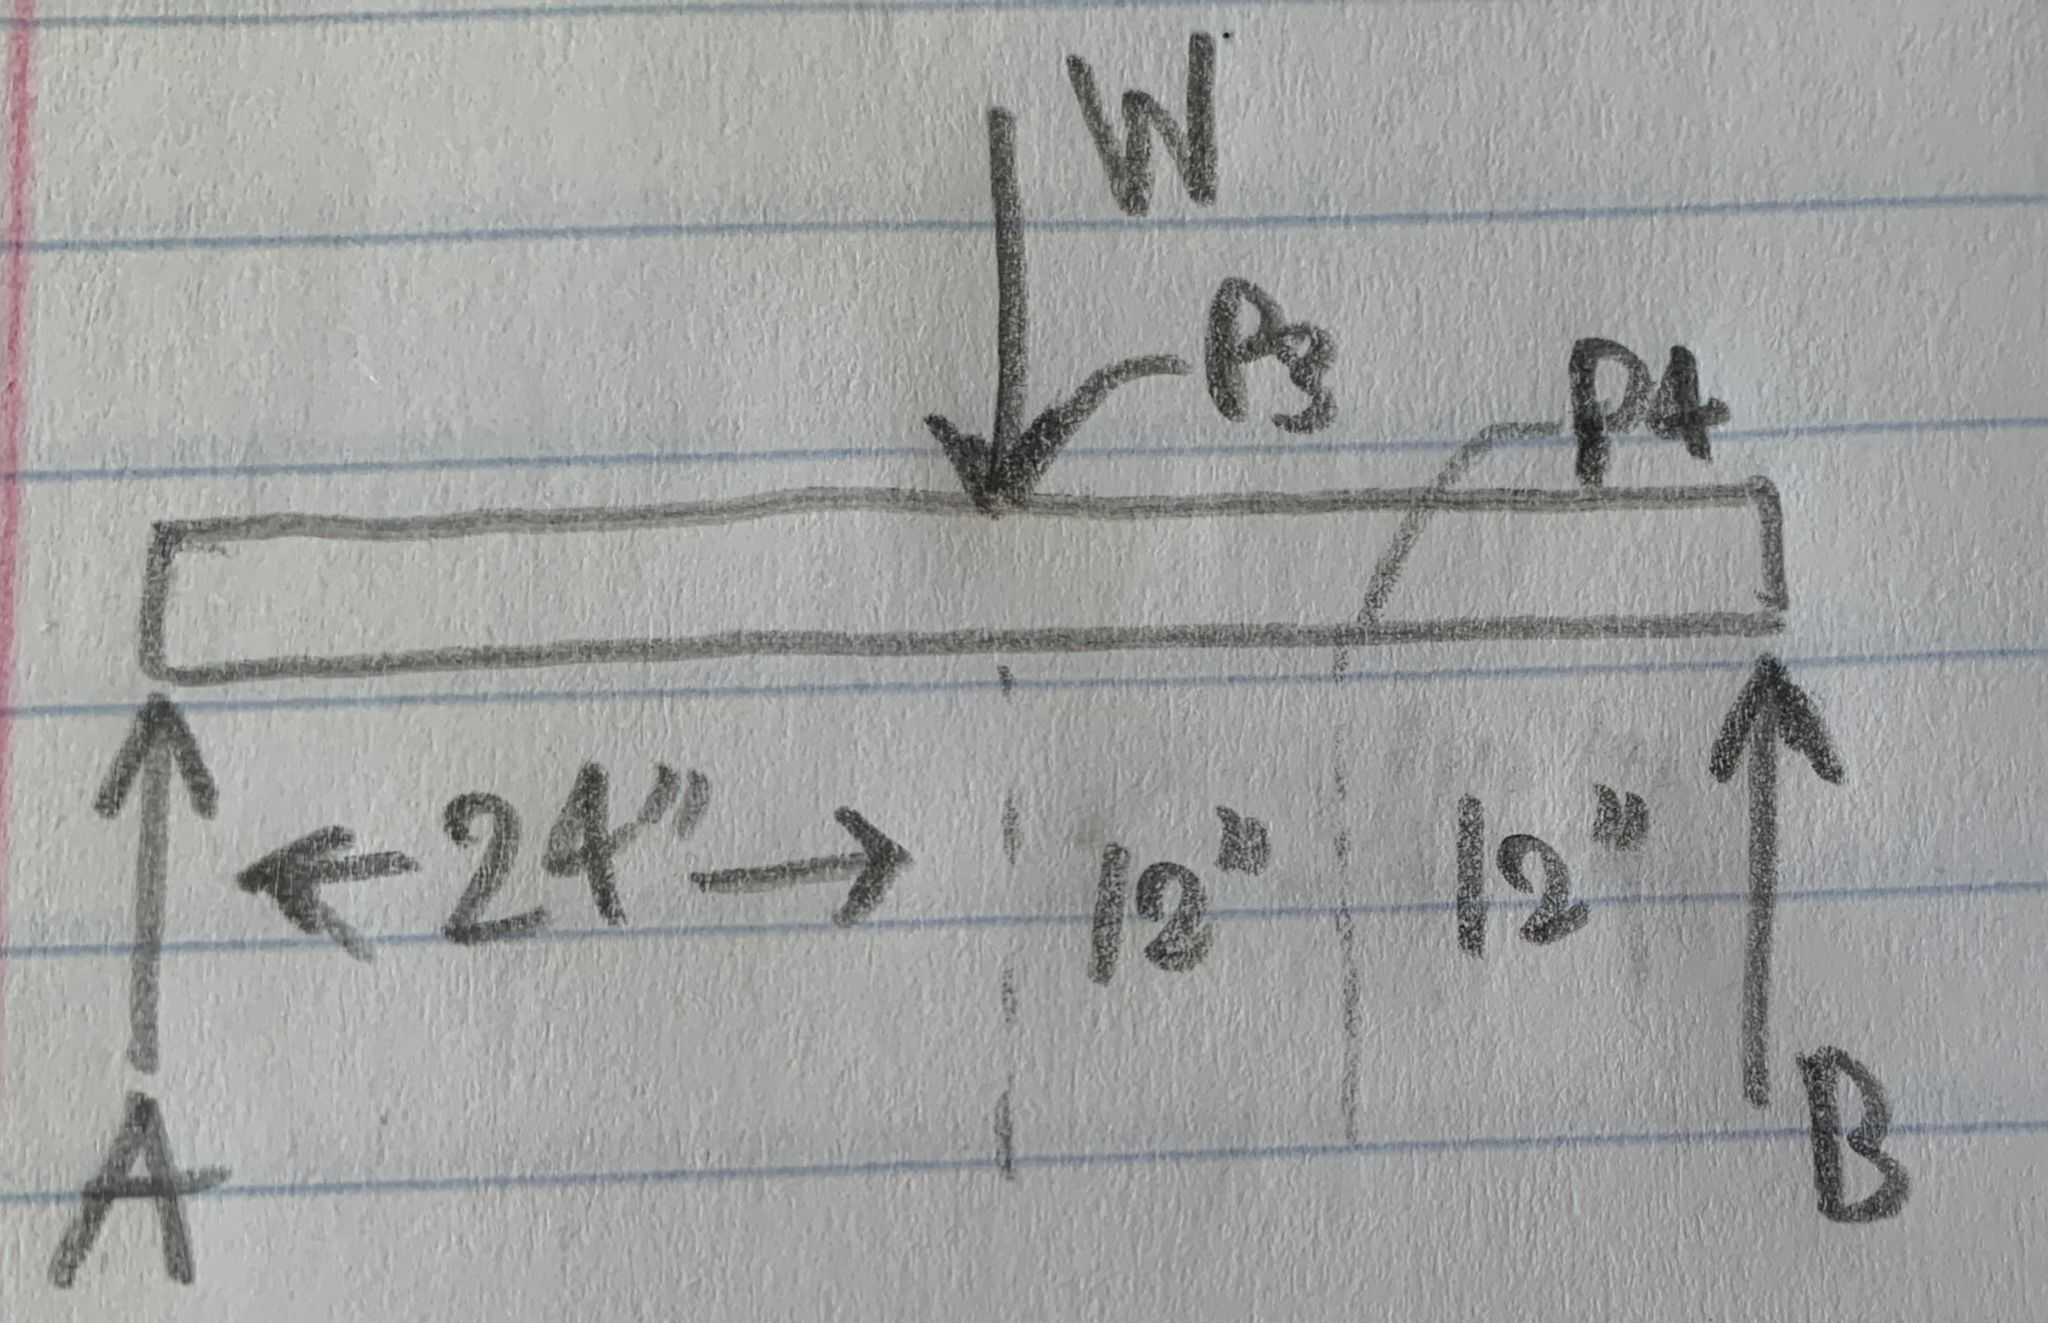
\includegraphics[width=0.6\textwidth]{./Images/S_mid.jpg}
    \caption{Free-body diagram of the simply supported beam with the load
    applied at the mid-span.}
    \label{fig:SimplySupportedBeamMid}
\end{figure}
\subsubsection{Simply Supported Beam Load Applied at the Quarter-Span}
\begin{figure}[H]
    \centering
    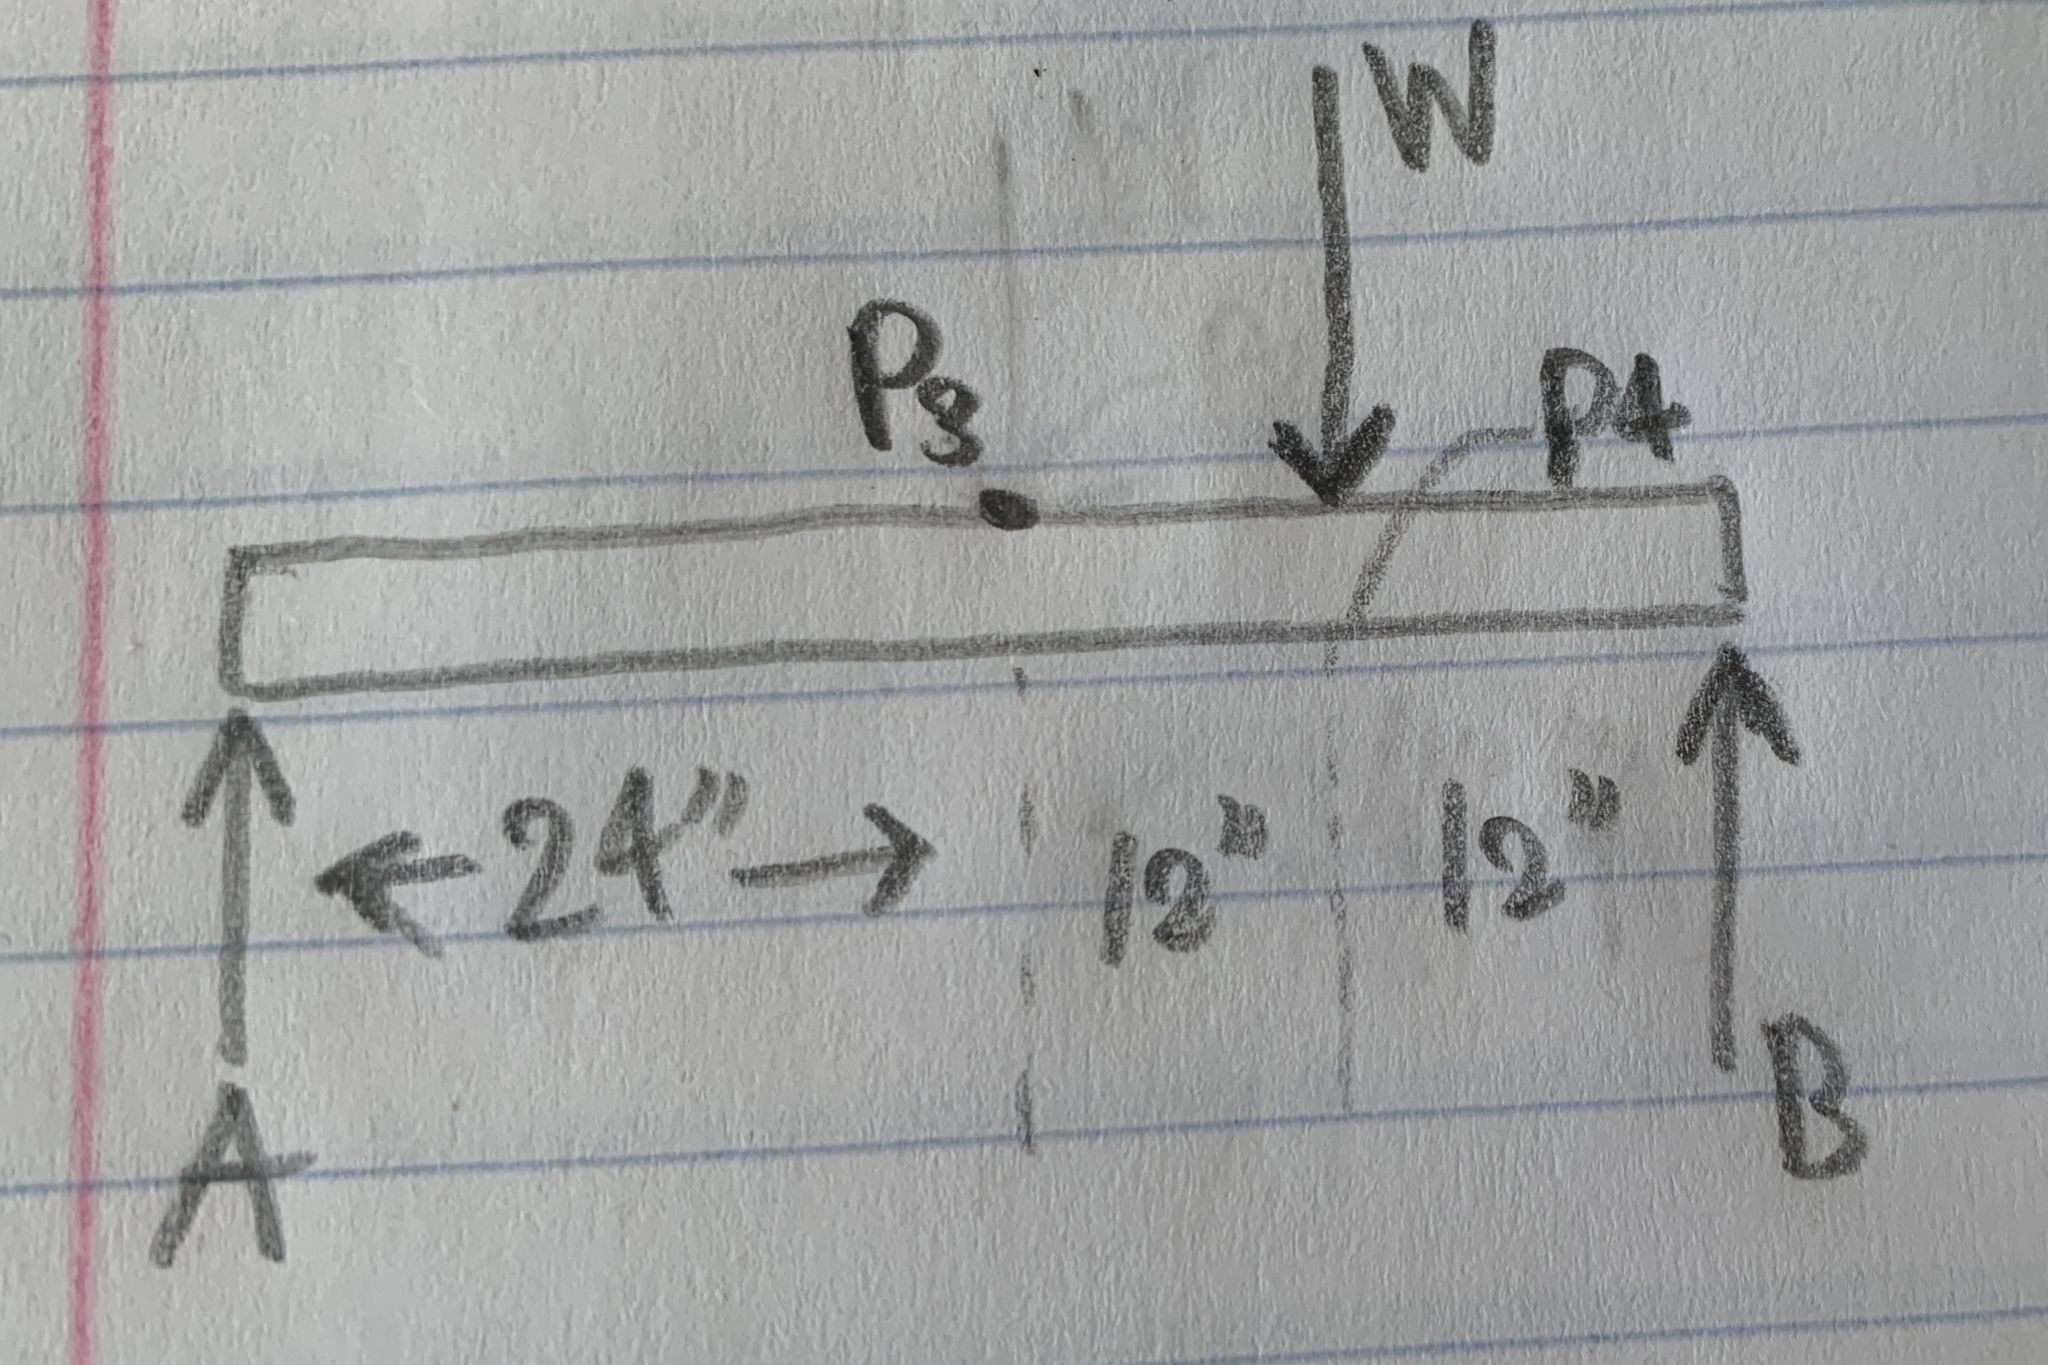
\includegraphics[width=0.6\textwidth]{./Images/S_quarter.jpg}
    \caption{Free-body diagram of the simply supported beam with the load
    applied at the quarter-span.}
    \label{fig:SimplySupportedBeamQuarter}
\end{figure}
\newpage
\section{Results}
\subsection{Cantilever Beam Load Applied at the End}
\subsubsection{Theoretical Results}
\subsubsection{Experimental Results}
\subsubsection{Comparison of Theoretical and Experimental Results}
\subsection{Cantilever Beam Load Applied at the Mid-Span}
\subsubsection{Theoretical Results}
\subsubsection{Experimental Results}
\subsubsection{Comparison of Theoretical and Experimental Results}
\subsection{Simply Supported Beam Load Applied at the Mid-Span}
\subsubsection{Theoretical Results}
\subsubsection{Experimental Results}
\subsubsection{Comparison of Theoretical and Experimental Results}
\subsection{Simply Supported Beam Load Applied at the Quarter-Span}
\subsubsection{Theoretical Results}
\subsubsection{Experimental Results}
\subsubsection{Comparison of Theoretical and Experimental Results}
\newpage
\section{Discussion}
\subsection{Analysis of Results}
\subsection{Sources of Error}
\newpage
\section{Conclusions}
\subsection{Summary}
\subsection{Maxwell's Law of Reciprocal Deflections}
\end{document}
